\documentclass{beamer}
\usepackage[utf8]{inputenc}
\usepackage{graphicx}
\usetheme{Madrid}

\title{Quantum Circuit Compilation for Trapped-Ion Processors\\with the Drive-Through Architecture}
\author{Cheming Chang, Jiehong roland Jiang, Dahwei Chiou, Ting Hsu, Guindar Lin}
\institute{Taipei, Taiwan}
\date{\today}

\begin{document}
	
	\begin{frame}
		\titlepage
	\end{frame}
	
	\begin{frame}{Introduction: Quantum Computing and Trapped-Ion Processors}
		\begin{itemize}
			\item Quantum computing exploits superposition and entanglement.
			\item Trapped-ion systems are one of the leading hardware platforms.
			\item Ions are confined in traps and manipulated with lasers.
			\item High-fidelity gates and long coherence times.
		\end{itemize}
	\end{frame}
	
	\begin{frame}{Introduction: Scalability Challenges}
		\begin{itemize}
			\item Single ion chains slow down as they grow.
			\item Modular approach: QCCD architecture shuttles ions between traps.
			\item Ion shuttling introduces latency, heat, and error.
		\end{itemize}
	\end{frame}
	
	\begin{frame}{Motivation: Drive-Through Architecture}
		\begin{itemize}
			\item Static qubits in traps, mobile communication qubits circulate on a racetrack.
			\item Reduces motional heating and re-cooling time.
		\end{itemize}
		\begin{figure}
			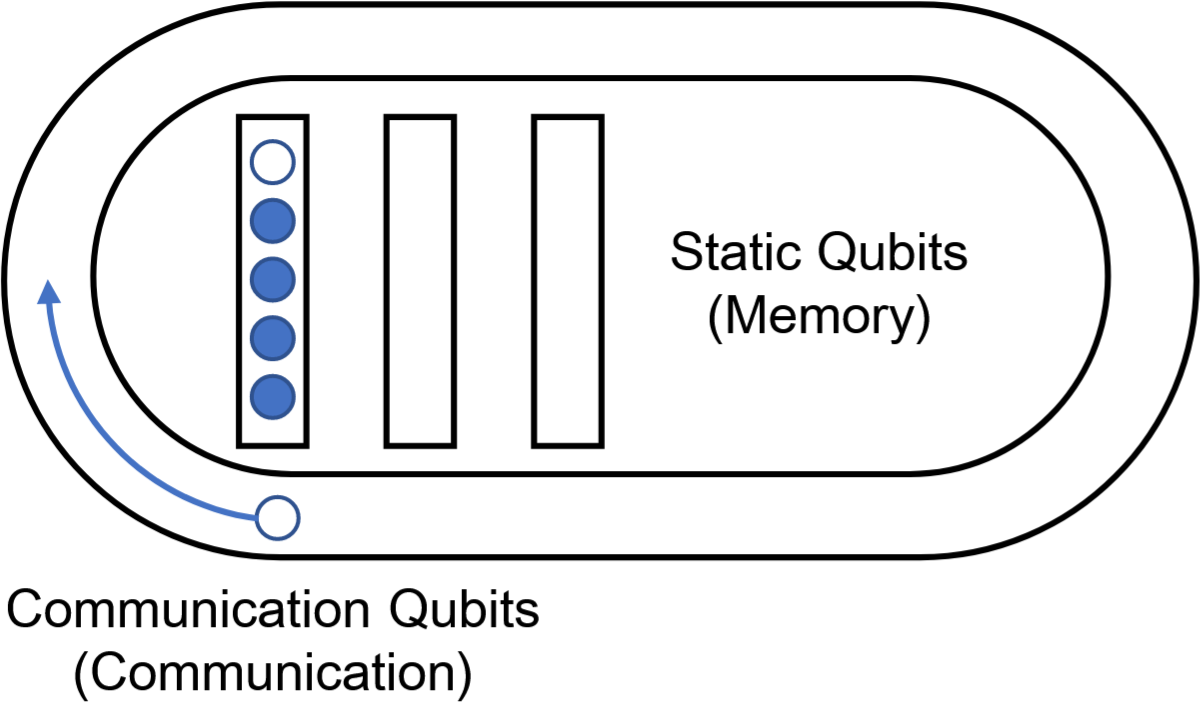
\includegraphics[width=0.6\textwidth]{figure/arch.png}
			\caption[]{The "drive-through" architecture with static qubits in traps and communication qubits on the racetrack. Some qubits may be information-free (colored in white)}
		\end{figure}
	\end{frame}
	
	\begin{frame}{Limitations and Challenges}
		\begin{itemize}
			\item Communication ions only connect to trap boundaries.
			\item Information must be swapped in and out.
		\end{itemize}
		\begin{figure}
			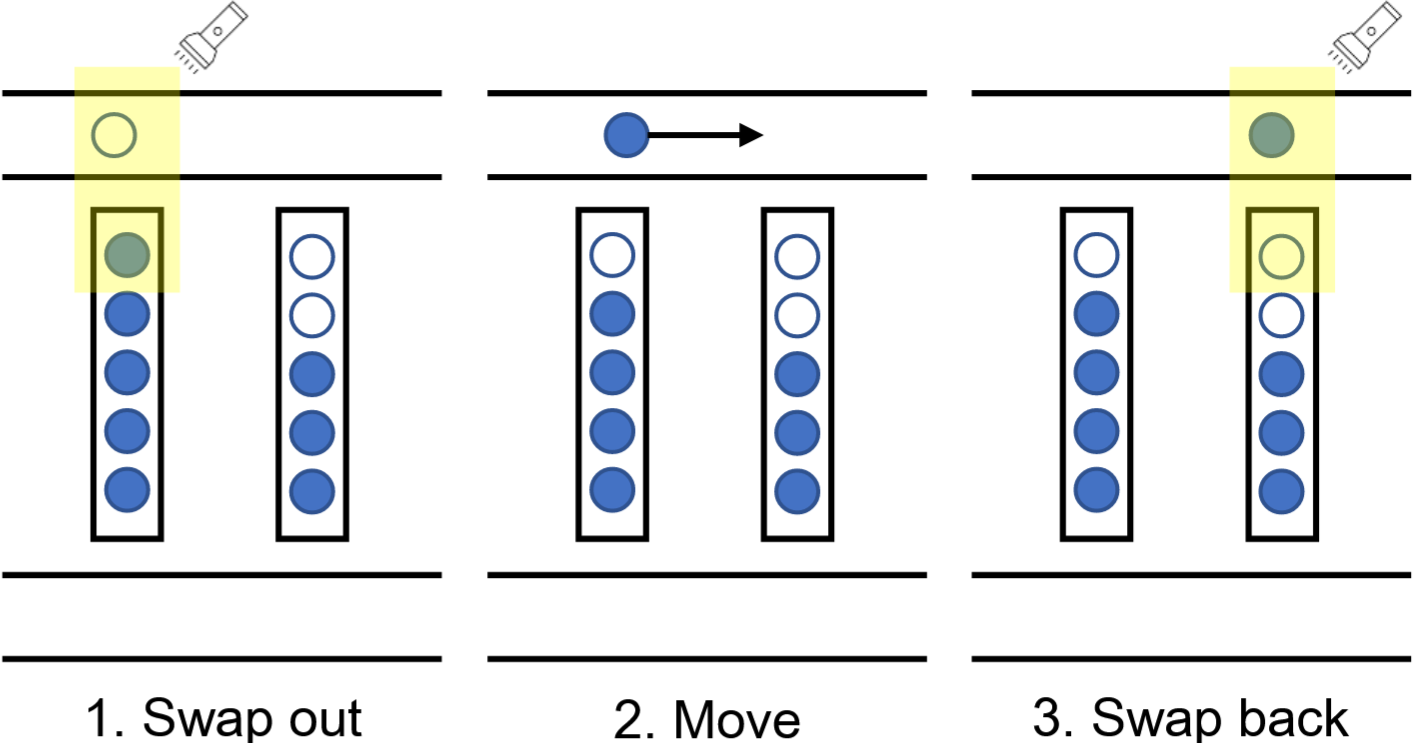
\includegraphics[width=0.8\textwidth]{figure/move.png}
			\caption[]{Methods for transporting the information of a static qubit to another trap.}
		\end{figure}
	\end{frame}
	\begin{frame}{Architecture graph}
		\begin{figure}
			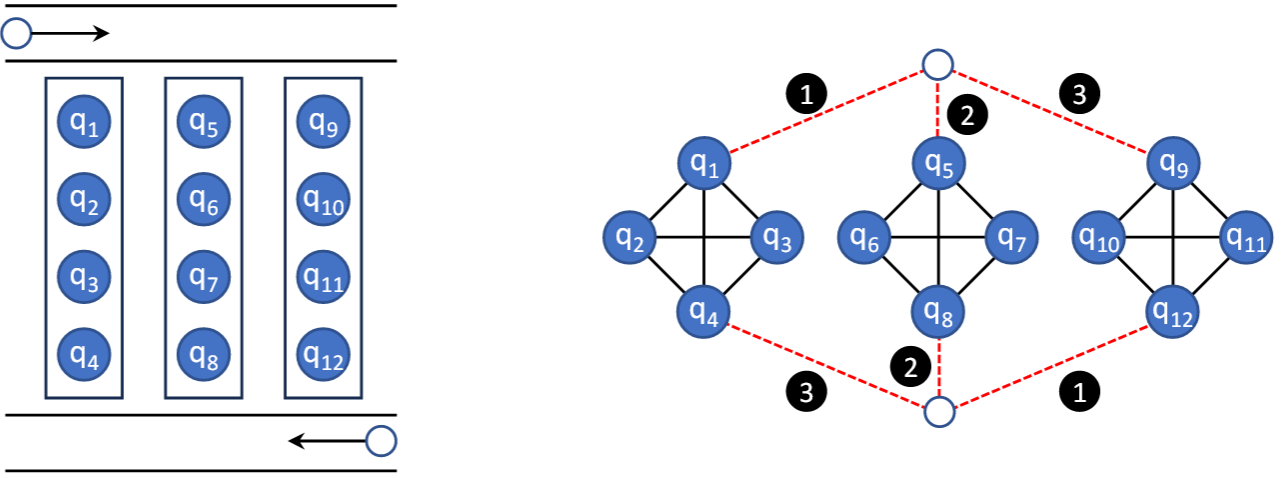
\includegraphics[width=.8\textwidth]{figure/graph.png}
			\caption[]{The drive-through architecture. Note that the communication edges in the drive-through architecture are available in specific orders.}
		\end{figure}
	\end{frame}
	\begin{frame}{Methods: Compiler Overview}
		\begin{itemize}
			\item Circuit \textrightarrow{} DAG \textrightarrow{} Gate partitioning \textrightarrow{} Qubit placement.
			\item Layer-wise processing with look-ahead.
			\item Optimize placement for fidelity and transport cost.
		\end{itemize}
	\end{frame}
	
	\begin{frame}{Gate Partitioning}
		\begin{itemize}
			\item Cluster qubits per layer using min-cut.
			\item Look-ahead mechanism for future gates. Adaptive window depth.
		\end{itemize}
		\begin{figure}
			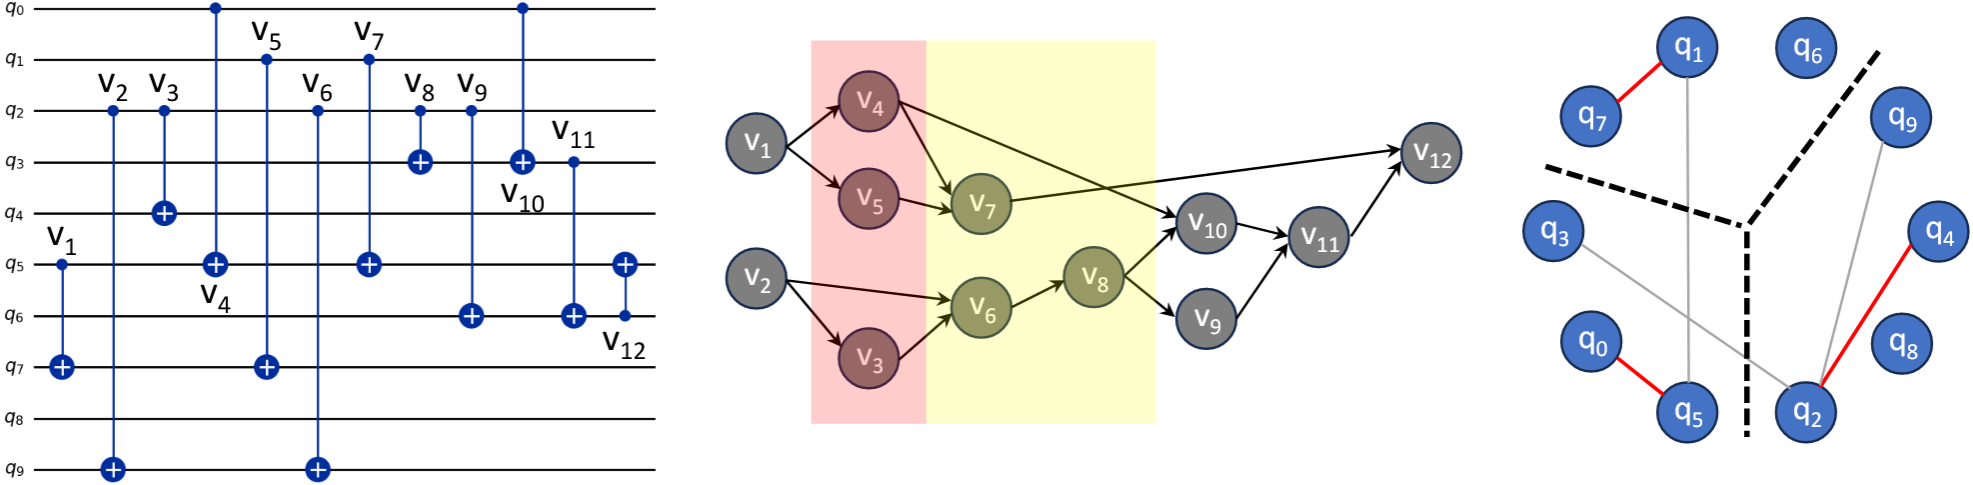
\includegraphics[width=\textwidth]{figure/cut.png}
			\caption[]{An illustration of circuit DAG generation and the gate partitioning at $\ell$ = 1}
		\end{figure}
	\end{frame}
	
	\begin{frame}{Dynamic Qubit Placement}
		\begin{itemize}
			\item Simulated annealing to minimize placement cost.
			\item Cost = Gate distance + 3*Swap penalty + Pull force.
		\end{itemize}
		\begin{figure}
			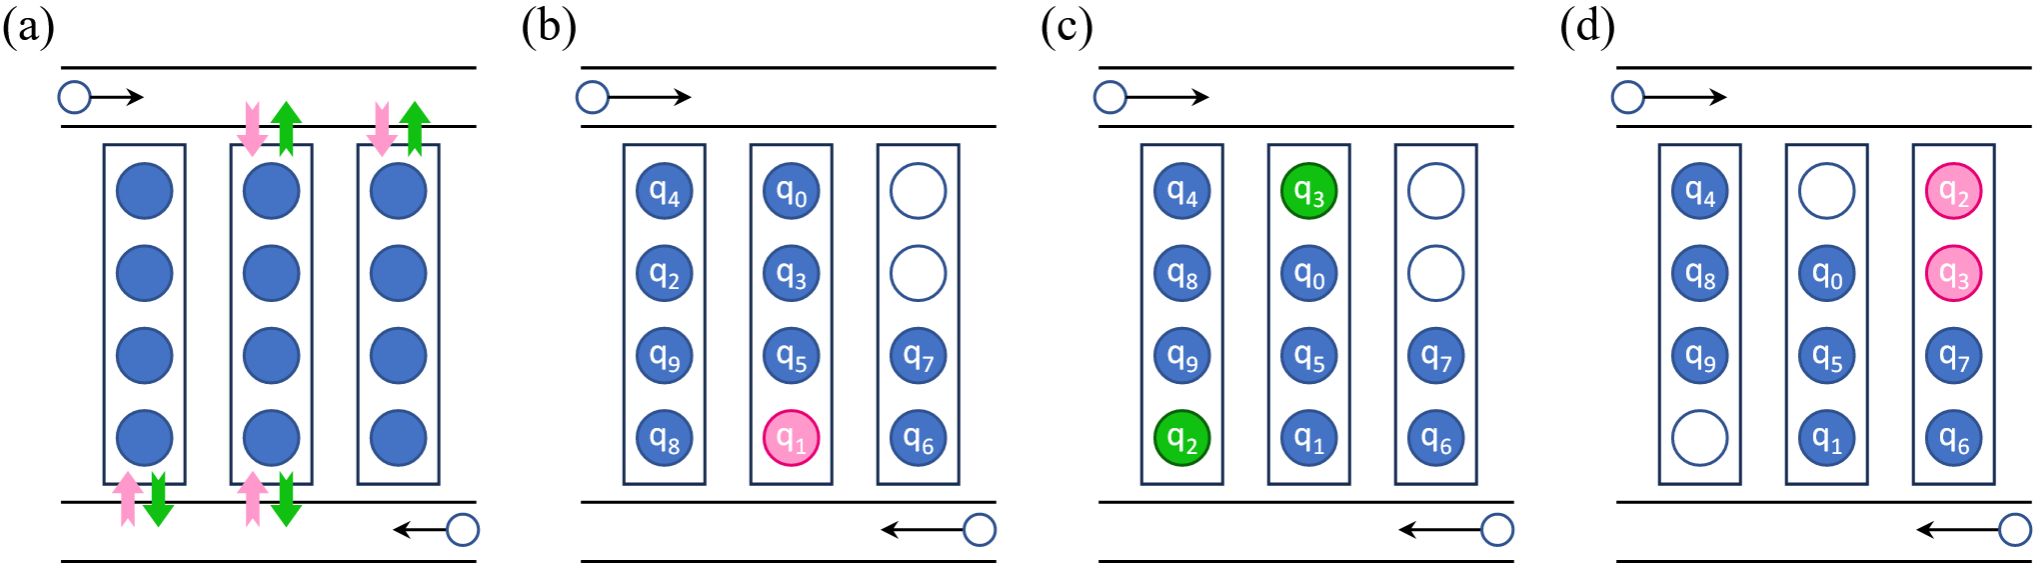
\includegraphics[width=.8\textwidth]{figure/qubit.png}
			\caption[]{An illustration of layer-wise placement}
		\end{figure}
	\end{frame}
	
	\begin{frame}{Distance function}
		\begin{itemize}
			\item The gate distance measures how far apart the qubits involved in two-qubit gates are within a trap.
			\[
			\text{gd}(\pi_{\ell,j}) = \sum_{q_m, q_n \in P_{\ell,j},(q_m, q_n) \in V_{G_{\ell}}} |\pi_{\ell,j}(q_m) - \pi_{\ell,j}(q_n)|
			\]
			\item The swap distance measures the number of swaps needed to transform the initial configuration $\pi_{\ell,j,0}$ to the optimized configuration $\pi_{\ell,j}$.
			\[
			\text{sd}(\pi_{\ell,j}, \pi_{\ell,j,0}) = \frac{1}{2} \sum_{i} |\pi_{\ell,j,0}(i) - \pi_{\ell,j}(i)|
			\]
			\item The boundary leaving cost.
		\end{itemize}
	\end{frame}
	\section{Results}
	\begin{frame}{Benchmark Circuits}
		\begin{itemize}
			\item Evaluated on QNN, QAOA, QFT, Quantum Volume, Random circuits.
			\item Compared against SABRE and t$|$ket$\rangle$.
		\end{itemize}
	\end{frame}
	
	\begin{frame}{Reduced Inter-Trap Communication}
		\begin{itemize}
			\item Example: Random circuit
			\item SABRE-ext: 10118 moves $\rightarrowtail$ 5979 moves.
			\item ~40\% reduction.
		\end{itemize}
		\begin{figure}
			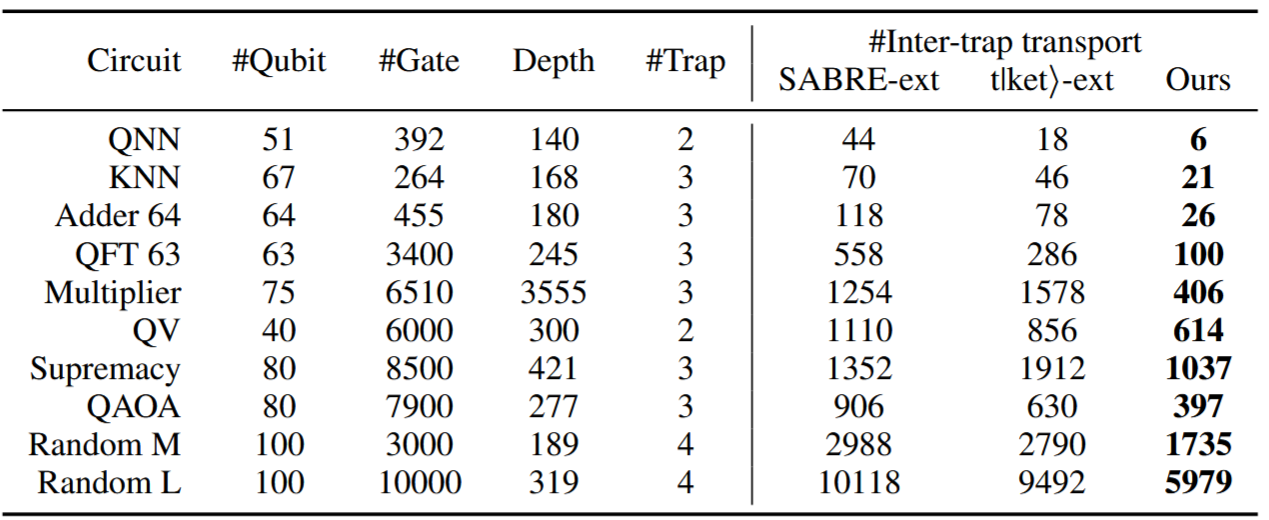
\includegraphics[width=.8\textwidth]{figure/com.png}
		\end{figure}
	\end{frame}
	
	\begin{frame}{Fidelity Improvements}
		\begin{itemize}
			\item Drive-through-aware compiler improves fidelity.
			\item Fewer ion swaps, reduced gate distance.
		\end{itemize}
		\begin{figure}
			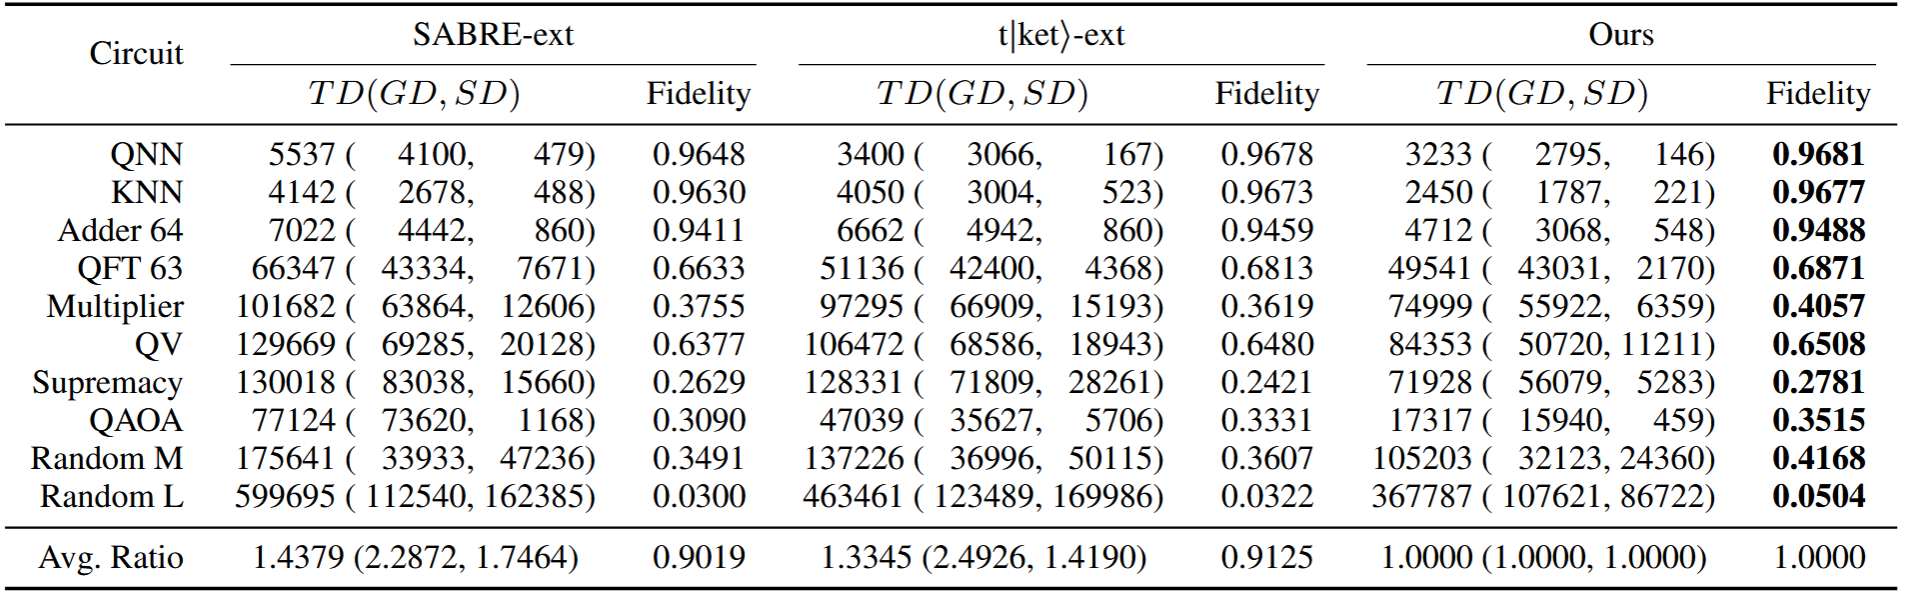
\includegraphics[width=.8\textwidth]{figure/fid.png}
		\end{figure}
	\end{frame}
	
	
	\begin{frame}{Scalability and Efficiency}
		\begin{itemize}
			\item Handles 100+ qubit circuits with thousands of gates.
			\item Quadratic scaling with circuit size.
		\end{itemize}
		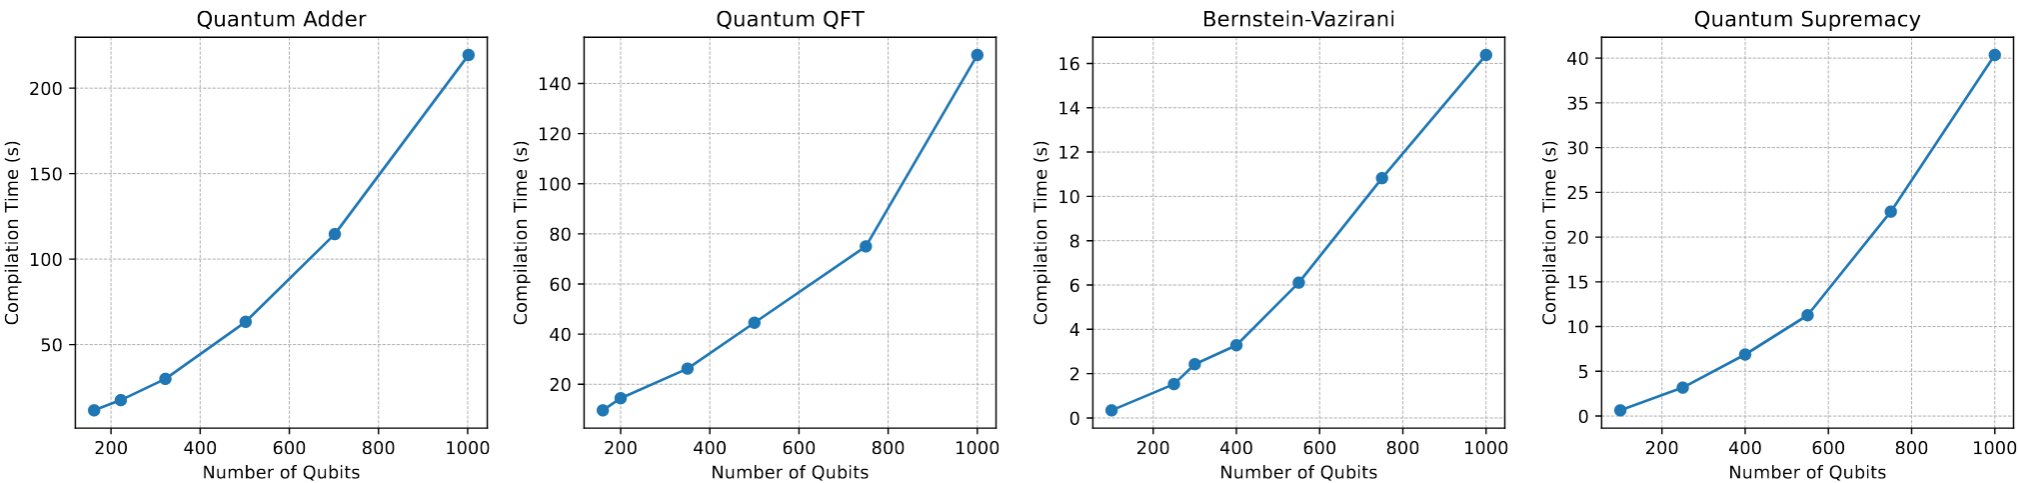
\includegraphics[width=\textwidth]{figure/time.png}
	\end{frame}
	
	\begin{frame}{Conclusion}
		\begin{itemize}
			\item Drive-through architecture enables low-overhead communication.
			\item Compiler maps circuits with higher fidelity and lower transport cost.
		\end{itemize}
	\end{frame}
	
\end{document}
